%% Exemplo de como usar a classe ppgccufscar.
%% O template da monografia (quali, dissertacao ou tese)
%% foi feito pela Profa. Sandra Fabbri.
%% A classe ppgccufscar foi feita por Daniel Beck,
%% Daniel Bruno e Prof. Marcio


%%
%% Opcoes que podem ser passadas 'a classe
%%
%% Todas as opcoes da classe abnt (AbnTeX) sao validas.
%% Outras opcoes sao: quali e tese (dissertacao e' padrao)
%%
\documentclass[quali]{ppgccufscar}

%% pacotes que deseja usar
%% pacotes incompativeis sao:
%%   qualquer pacote de citacoes, como natbib, apalike, cite, etc.
%% o pacote babel ja vem carregado com ingles e portugues
%\usepackage[latin1]{inputenc}
%\usepackage[brazilian]{babel}
\usepackage[utf8]{inputenc}
\usepackage[dvipdfm]{graphicx}
\usepackage{amsmath}
\usepackage{multirow}
\usepackage{url}

\graphicspath{{figuras/}}

% Change these to change out the sort outputs.

\titulo{Metodologias de desenvolvimento de jogos eletrônicos: Um estudo comparativo}
\autor{Erick Vansim Previato}
\orientador[Orientador]{Prof. Dr. Delano Medeiros Beder}
\areaconcentracao{Engenharia de Software}
\data{Novembro/2016}

% epigrafre, agradecimentos sao feitos 'na mao'.
% um dia eu faco alguns comandos para eles ;)

\begin{document}

\capa
\folhaderosto

\dedicatoria{A meus pais e minha namorada.}
%\begin{agradecimentos}
%
%\end{agradecimentos}

\epigrafe{Gostaria de uma sociedade mais justa, menos corrupta, com menos hipocrisia, mais digna, 
com mais amor ao próximo, menos preconceito, menos rancor e principalmente mais paz na alma.}{Albert Einstein}

\begin{resumo}
A competitividade no mercado de jogos sempre foi alta, com isso, empresas buscam a todo tempo adotar metodologias de desenvolvimento que aumentem a produtividade e a interação da equipe, diminua o gasto e o tempo de desenvolvimento, tudo isso sem perder a qualidade do produto final. O processo de desenvolvimento de jogos não é algo tão simples como o desenvolvimento de um sistema de informação, uma equipe de desenvolvimento de jogos precisa ser multidisciplinar, pois para desenvolver um jogo existem etapas que necessitam de pessoas que não são necessariamente da área da computação como artista, engenheiro de áudio, roteirista, entre outros. Pensando nessa especificidade de desenvolvimento de jogos, este trabalho propõe um estudo comparativo entre as metodologias de desenvolvimento voltadas para jogos existentes na literatura, e contrapôr com as metodologias que são utilizadas na prática por empresas e grupos de pesquisa da região de São Carlos, e que tenham como foco principal o desenvolvimento de jogos. Como resultado espera-se gerar uma documentação de tendências de metodologias e artefatos voltadas para o desenvolvimento de jogos, além de sugerir propostas de melhorias das metodologias ou métricas utilizadas nesse cenário.
\palavraschave{Metodologias, Desenvolvimento, Jogos eletrônicos}
\end{resumo}

\begin{abstract}
The competition in the game market has always been high, with this, companies seek at all times to use development methodologies that increase productivity and team interaction, decrease the cost and development time, all without losing the quality of the final product. The game development process is not as simple as the development of an information system, a game development team must be multidisciplinary, because to develop a game there are steps that need people who are not necessarily of computer area as artist, audio engineer, writer, among others. Thinking that game development specificity, this paper proposes a comparative study of the development methodologies focused on existing games in the literature, and compare with the methodologies that are used in practice by companies and research groups of the São Carlos region, and whose main focus on game development. As a result is expected to generate a documentation of trends of methodologies and artifacts focused on the game development, and suggest proposals for improvement of the methodologies and metrics used in this scenario.
\keywords{Methodologies, Development, Eletronic Games}
\end{abstract}

\listoffigures
\listoftables

%% de acordo com o template, o glossario vem
%% depois das referencias e deve estar em ordem
%% alfabetica.
%% depois de muito esforco consegui fazer com que
%% o glossario ficasse em ordem alfabetica automaticamente.
%% ainda nao sei a escalabilidade do algoritmo :(

%% DICA: voce pode ir definindo os acronimos ao longo do texto.
%% Por exemplo, no capitulo 1, vc ta escrevendo:
%% Segundo Fulano, Model-Driven Development (MDD)\acronym{MDD}{Model-Driven Development} é uma técnica bla bla bla...

\acronym{RUP}{Rational Unified Process}
\acronym{UML}{Unified Modeling Language}
\acronym{TDD}{Test-Driven Development}
\acronym{FDD}{Feature-Driven Development}
\acronym{DSDM}{Dynamic Systems Development Method}
\acronym{XP}{Extreme Programming}
\acronym{XGD}{Extreme Game Development}
\acronym{GUP}{Game Unified Process}
\acronym{TI}{Tecnologia da Informação}
\acronym{AGP}{Agile Game Process}

\listofacronyms

%% sumario
\tableofcontents

%% aqui comeca o texto da monografia
%% voce pode dividir o conteudo em varios arquivos.
%% por exemplo, intro.tex, fundamentacao.tex, desenvolvimento.tex, conclusao.tex.
%% dai, vc inclui aqui assim: \input{intro.tex} e assim por diante.




\chapter{Introdução}

\section{Contextualização}

Com os recentes avanços na última década, inúmeros aparatos tecnológicos têm sido desenvolvidos pela indústria, setores privados ou propostos pela academia científica. Em específico, a computação tem ajudado no desenvolvimento de tais soluções, tanto no domínio de hardware quanto no de software.

No contexto de software, as soluções envolvem aplicações na área da medicina como softwares para diagnósticos, para acompanhamento de tratamento de pacientes, entre outros \cite{sommerville2010}; na área de engenharia civil com softwares e aplicações para cálculos e projeções de custos e riscos \cite{ribeiro2016}; na área financeira com sistemas de projeções de cálculos de inflações, juros, e outros \cite{costa2012}; até a recente área denominada Big data, na qual uma quantidade massiva de dados é gerenciada \cite{hp2016}.

Dentre todas as aplicações existentes, tem-se uma crescente demanda no desenvolvimento de jogos digitais, seja para os vários tipos de consoles eletrônicos, seja para computadores tradicionais ou para o atual mercado de smartphones.

No começo do mercado de desenvolvimento de jogos, equipes eram pequenas, projetos não eram tão grandes e as plataformas que rodavam esses jogos não eram tão vastas. Com o passar dos anos a complexidade dos jogos aumentou e, portanto, fez-se a necessidade de utilizar equipes cada vez maiores e multidisciplinares, a considerar-se que tais jogos devem ser desenvolvidos para uma vasta gama de dispositivos, desde consoles tradicionais até smartphones.

Como a competitividade nesse mercado de jogos sempre foi alta, empresas buscam a todo tempo adotar metodologias de desenvolvimento que aumentem a produtividade e a interação da equipe, diminua o gasto e o tempo de desenvolvimento, tudo isso sem perder a qualidade do software, neste caso os jogos digitais.

Assim como adotado em desenvolvimento de softwares no geral, é necessário adotar uma abordagem eficiente e eficaz para o desenvolvimento de softwares desse gênero. Para isso será abordado neste trabalho algumas metodologias de desenvolvimento de software e sua utilização e aceitação no mercado atual.

Na literatura existem adicionalmente inúmeras abordagens e metodologias descritas. Na engenharia de software é comumente estabelecido o modelo de desenvolvimento denominado cascata, também conhecido como modelo tradicional. Este modelo visa elaborar um projeto de uma forma sequencial, onde as etapas são pré-definidas como levantamento de requisitos, projeto, implementação, testes e validação e, por fim, a manutenção \cite{sommerville2010}.

Uma abordagem de desenvolvimento de software em evidência no contexto atual é conhecida como metodologia ágil, que por sua vez surgiu em 2001 quando um grupo de especialistas trocaram experiências e estabeleceram alguns princípios e valores, criando assim o manifesto ágil: “O Manifesto Ágil é uma declaração sobre os princípios que servem como base para o desenvolvimento ágil de software” \cite{beck2001}.

Na atualidade, várias empresas estão utilizando metodologias ágeis em seus projetos, pois a aceitação e o índice de sucesso tem aumentado durante os últimos anos. De acordo com \citeonline{hastie2015}, um relatório denominado \textit{Chaos Report} tem sido publicado desde 1994 por Standish Group \footnote{Mais informações sobre Standish Group podem ser encontradas no site: https://www.standishgroup.com/about}. No relatório de 2015 foram analisados 50 mil projetos ao redor do mundo, e constatou-se que apenas $29\%$ dos projetos tiveram sucesso nos últimos 5 anos. Dentro dessa análise ainda, destaca-se uma comparação feita com projetos que utilizaram metodologia tradicional e os que utilizaram metodologia ágil, onde a porcentagem de sucesso com metodologia ágil é de $39\%$, e na metodologia tradicional apenas $11\%$. Existem vários fatores envolvidos nessa pesquisa, como tamanho e complexidade dos projetos, mas o resultado mostra que as metodologias ágeis vem conquistando cada vez mais o mercado de desenvolvimento.


\section{Objetivo}

O objetivo principal desta pesquisa é levantar dados relacionados às metodologias de desenvolvimento de jogos e artefatos encontrados na literatura em consonância com os padrões utilizados pelas empresas de desenvolvimento de jogos da cidade de São Carlos e região, a fim de obter dados que auxiliem pesquisadores e desenvolvedores de jogos a desenvolverem produtos mais eficientes com melhor custo/benefício.
 

\section{Organização}

No Capítulo \ref{cap_2} será abordado uma breve introdução da realidade do mercado de TI, alguns conceitos fundamentais sobre desenvolvimento de jogos e também sobre as metodologias de desenvolvimento, além de alguns trabalhos relacionados; No Capítulo \ref{cap_3} será apresentado o desenvolvimento do trabalho e um cronograma de atividades proposto para conclusão da pesquisa.

%Exemplo de citação indireta \cite{tolvanenKelly08}.
%Exemplo de citação de autor: Segundo \citeonline{lucredio2009}, bla bla bla.
%Exemplo de citação longa:

%\begin{citacao}
%A teleconferência permite ao indivíduo participar de um encontro
%nacional ou regional sem a necessidade de deixar seu local de
%origem. Tipos comuns de teleconferênia incluem o uso da televisão,
%telefone e computador. Através de áudio conferência, utilizando
%a companhia local de telefone, um sinal de áudio pode ser emitido
%em um salão de qualquer dimensão \cite[p. 181]{weberZhang96}.
%\end{citacao}




\chapter{Conceitos fundamentais}
\label{cap_2}


\section{Considerações iniciais}

Este capítulo trata de conceitos fundamentais e metodologias necessários para a realização deste projeto de pesquisa. A sequência deste capítulo segue com um estudo geral sobre a área de desenvolvimento de software e sua realidade atual no mercado. Em seguida, são abordados e apresentados os principais conceitos e definições sobre o tema de desenvolvimento de jogos. Após, tem-se uma descrição sobre as metodologias de desenvolvimento de software e sua utilização no cenário de jogos, fazendo uma análise mais aprofundada sobre a metodologia tradicional, RUP e algumas das metodologias ágeis. Um breve estudo sobre métricas e sobre os trabalhos relacionados também é apresentado. Por fim, são apresentadas as considerações finais ao fim do capítulo.


\section{Realidade do mercado de TI}
\label{sec_mercado}

Nos dias atuais é inegável que o uso de sistemas de informação dos mais variados tipos tem uma grande importância para o sucesso de qualquer instituição, seja ela pública ou privada. Essa crescente busca pelo uso de sistemas informatizados, tem exigido cada vez mais resultados positivos com menos investimento e mais retorno \cite{roberts2011}. 

Vários fatores tornam o desenvolvimento de software uma tarefa não trivial. As principais  dificuldades encontradas na entrega do produto podem ser, por exemplo, compreender e encontrar uma maneira concisa e clara para representar o que o cliente realmente deseja, quais tecnologias e metodologias a utilizar, como estimar tempo e custo, mudanças de normas e legislações, entre outros fatores.

Baseando-se em três pilares para avaliar o sucesso do produto (tempo, orçamento e qualidade), o relatório \textit{Chaos Report} é amplamente utilizado na literatura. De acordo com \citeonline{hastie2015}, que analisaram os dados de 2015, foram avaliados cerca de 50.000 projetos ao redor do mundo entre 2011 e 2015. Os resultados mostram que apenas $29\%$ foram concluídos com sucesso, $52\%$ tiveram alguma mudança de requisitos ou de funcionalidades, ou tiveram alterações de prazo ou custo, e $19\%$ não chegaram a se tornar um produto de fato.

Como visto, uma boa parte dos projetos apresentam algum tipo de dificuldade em alguma parte do processo de desenvolvimento. Geralmente, essas dificuldades transformam-se em prejuízos tanto para o cliente quanto para o empreendedor. Vale ressaltar que, atualmente é comum encontrar equipes multidisciplinares envolvidas em um mesmo projeto, o que pode tornar-se um problema se não houver comunicação clara e objetiva entre elas.

A necessidade de eliminar os  fatores que de alguma maneira influenciam negativamente no desenvolvimento de um projeto torna-se indispensável na área de engenharia de software. Nesse sentido, destaca-se a importância da utilização de uma metodologia de desenvolvimento que norteie o processo de construção do projeto de software, que por sua vez, contêm um conjunto de diretrizes, conceitos e padrões a serem seguidos.

Na Seção \ref{sec_metodologias} apresenta-se uma discussão sobre as metodologias utilizadas atualmente no desenvolvimento de software e suas aplicações no desenvolvimento de jogos eletrônicos.


\section{Desenvolvimento de jogos}
\label{sec_jogos}

O processo de desenvolvimento de jogos eletrônicos não é um procedimento simples, além disso, é comum alguns desenvolvedores começarem o desenvolvimento de um jogo sem utilizar etapas ordenadas, sem seguir um método e sem o devido cuidado para gerar o conceito do jogo \cite{schuytema2006,novak2012}. Essa falta de uma metodologia pode resultar em falta de público alvo definido, falta de foco, falhas de desenvolvimento, entre outros problemas.

Como visto na seção anterior a aplicação de uma metodologia de desenvolvimento é muito importante para o desenvolvimento de um software, e isso também se aplica no setor de jogos eletrônicos. Na literatura encontram-se algumas etapas para o desenvolvimento de jogos eletrônicos, um modelo para tentar evitar os problemas mais comuns encontrados no processo de desenvolvimento de jogos. Segundo \citeonline{novak2012}, o processo de desenvolvimento de jogos engloba as seguintes etapas:

\begin{itemize}
	\item Conceito: para essa etapa inicial, normalmente a equipe não é muito grande, podendo conter apenas alguns membros. O objetivo principal dessa equipe é criar a ideia do jogo. Além disso, também precisam identificar o público-alvo, avaliar se o jogo terá um mercado potencial e verificar os recursos disponíveis para tal construção. Como resultado dessa etapa é gerado o documento de conceito, que será utilizado para transmitir a ideia para outras pessoas envolvidas no projeto.
	\item Pré-Produção: tendo o conceito do jogo pronto, é necessário planejar todo o desenvolvimento, esse planejamento é conhecido como pré-produção. Nessa etapa, dois documentos são elaborados, um deles é o documento de design do jogo (\textit{Game Design Document}), que será utilizado como referência em todo o desenvolvimento do projeto, e o outro é o documento técnico de design (\textit{Technical Design Document}), que é baseado no documento de design do jogo e descreve os aspectos tecnológicos necessários para o desenvolvimento do projeto.
	\item Protótipo: o protótipo tem como principal função apresentar o funcionamento do jogo, mostrando o modo de jogar, e se o mesmo é atraente e divertido. Tal protótipo pode ser criado de maneira não digital, ou seja, utilizando painéis, papéis, cartões, entre outros, podendo ser uma maneira mais barata e rápida de visualizar a jogabilidade do projeto. Entretanto, um protótipo digital é muito importante para o desenvolvimento do jogo, pois pode ser um item fundamental para a decisão de levar ou não o projeto a frente. Além disso, quando se tem uma fonte financiadora por trás do projeto, geralmente é mais profissional apresentar um protótipo de um jogo em formato digital do que em papel.
	\item Produção: é a etapa mais extensa do projeto, é onde o jogo é de fato desenvolvido. Normalmente esta etapa dura de 6 a 24 meses, e só acaba quando o jogo puder ser testado do começo ao fim. Cabe ressaltar nessa etapa a importância do acompanhamento dos gerentes e supervisores, pois quando se tem um prazo muito apertado, o time pode sofrer com pressões desnecessárias, gerando assim uma desmotivação da equipe. Por outro lado, um prazo muito flexível, pode ser que a equipe comece o trabalho em um ritmo mais lento que o normal, ocasionando um trabalho excessivo ao final do projeto. O que auxilia esse acompanhamento, é a documentação e o planejamento realizado nas etapas anteriores.
	\item Fase alfa: como dito anteriormente, nessa etapa o game já pode ser jogado do início ao fim. Talvez os detalhes visuais tenham que ser melhorados, mas o funcionamento do jogo tem que estar completo. Nesta etapa a equipe de testes realiza os testes necessários em cada módulo pelo menos uma vez, e armazena todos os dados importantes de resultados e defeitos encontrados, gerando um documento chamado de plano de testes. Aqui também podem ser incorporados testadores de jogabilidade a fim de encontrar o maior número de problemas.
	\item Fase beta: o objetivo principal dessa etapa é estabilizar o projeto e focar na correção de problemas encontrados na etapa anterior. Outros testes são efetuados nessa etapa a fim de garantir a jogabilidade do jogo e identificar e corrigir problemas de desempenho. Após todas as correções é realizado a preparação do produto final. Para passar para a próxima fase, o código, o conteúdo, a interface com o usuário, a compatibilidade com hardwares e softwares, a arte e o áudio e o manual do jogo devem estar concluídos.
	\item Fase ouro: nesta etapa, depois de testado nos mínimos detalhes, o jogo é enviado ao fabricante para que avalie a base de defeitos e dê o aval de que o jogo está pronto. A partir daí o jogo começa a ser fabricado, onde a mídia é gerada e embalada. Ao sair da fase ouro, o jogo é lançado no mercado, e entra na etapa de pós-produção. A fase de fabricação pode ser eliminada se o jogo for comercializado online.
	\item Pós-Produção: conhecida também como pós-lançamento, é onde podem surgir outras versões do jogo, seja para melhorar ou substituir o mesmo. Tais versões ocorrem para sanar problemas pequenos no software, podendo ser falhas de programação ou até mesmo ajustes de configurações em hardwares não previstos. Outro ponto são as atualizações que podem aparecer para aprimorar o jogo, a fim de aumentar a vida útil do mesmo. Ambos são distribuídos gratuitamente para quem já possui o jogo.
\end{itemize}

Outros autores definem esse processo de desenvolvimento de jogos em menos etapas que essas descritas por \citeonline{novak2012}. \citeonline{rabin2} define o processo em 4 etapas: conceito, pré-produção, produção e pós-produção. Porém, as fases alfa e beta são encontradas dentro da etapa de produção, e o equivalente a etapa ouro está descrito na etapa de pós-produção. Já \citeonline{schuytema2006}, define o processo em apenas 3 etapas: pré-produção, produção e pós-produção. Nesse caso a etapa de conceito está abordada dentro da pré-produção, e as etapas alfa, beta e ouro dentro da produção. Mesmo com quantidade diferentes de etapas, há um consenso sobre o processo de desenvolvimento de jogos.

A Figura \ref{fig_jogos} apresenta as etapas do desenvolvimento de jogos, e seus respectivos documentos criados em cada etapa, conforme descrito anteriormente.

\begin{figure}[!htbp]
	\begin{center}
	\caption{Etapas do desenvolvimento de jogos segundo \citeonline{novak2012}}
	\label{fig_jogos}
	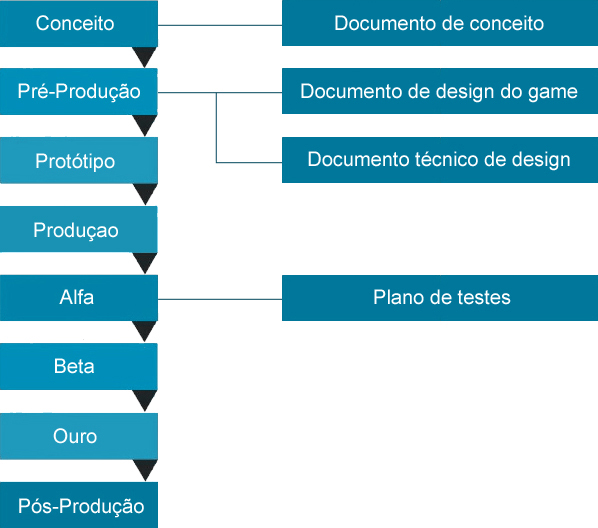
\includegraphics[width=0.6\textwidth,natwidth=598,natheight=528]{figura0.jpg}
	\end{center}
\end{figure}

Para desenvolver todo o processo de jogos, é necessário ter uma equipe bem definida, e dependendo do tamanho da equipe, pode ser que a mesma pessoa exerça o papel de mais de um dos descritos abaixo \cite{novak2012}:

\begin{itemize}
	\item Produtor: um dos principais objetivos do produtor é saber lidar com pessoas, é ele o responsável por solucionar conflitos, comunicar-se com clareza, gerenciar pessoas e ensinar a metodologia que será utilizada. O produtor portanto, é quem garante que o jogo será lançado dentro do prazo, com os recursos necessários, com a melhor qualidade possível, e que toda equipe esteja de fato envolvida no projeto. 
	\item Designer de jogos: é responsável por pensar no modo de jogar, na usabilidade, na navegação da interface e nos níveis do jogo, ou seja, garantir que o fator diversão esteja bem encaminhado. Criatividade nessa função é um fator muito importante, uma vez que não é fácil pensar em como um jogo será visto por outras pessoas.
	\item Artista: a função do artista é garantir que todo o material artístico do jogo seja elaborado, o que inclui objetos de cena, personagens, interiores, exteriores, veículos, entre outros. Geralmente são divididos em artista bidimensional (cria e refina elementos artísticos como personagens, objetos, interfaces, etc) e tridimensional (cria e refina elementos como texturas, iluminação, mapeamentos, etc). 
	\item Programador: o programador pode atuar em várias partes de um jogo, seja no banco de dados da aplicação, na programação de áudio, no motor do jogo (que seria o código principal), na programação gráfica, na programação de rede (se o jogo for online) até na programação de inteligência artificial. É responsável por dar vida ao jogo, de colocar toda ideia, artefatos e materiais artísticos em funcionamento.
	\item Áudio: nessa área, pode-se encontrar engenheiro/diretor de áudio, compositor, dublador ou designer de som. Basicamente esse profissional é responsável pelo áudio de um jogo, o que inclui efeitos sonoros, sons ambientes, diálogos e trilhas sonoras. Ele trabalha em conjunto com artistas e programadores a fim de garantir que tais elementos de áudio sejam inseridos corretamente no jogo.
	\item Controle de qualidade: conhecido também como testador, é o responsável por garantir a qualidade do jogo, que consiste em analisar as funcionalidades, a usabilidade e a lógica do jogo. Cabe ao mesmo determinar se o jogo é consistente, divertido e livre de erros, garantindo assim a jogabilidade do mesmo.
\end{itemize}

Após essa síntese apresentada sobre o desenvolvimento de jogos, nas próximas seções serão abordados detalhes sobre metodologias de desenvolvimento de software e como são aplicadas no desenvolvimento de jogos.


\section{Metodologias de desenvolvimento}
\label{sec_metodologias}

Como mencionado na Seção \ref{sec_mercado}, o uso de uma metodologia de trabalho para o desenvolvimento de software tem como objetivo ordenar e melhor gerenciar o processo de construção, tornando essa tarefa menos complicada \cite{sommerville2010,pressman2005}. 

Na literatura, o termo metodologia é amplamente utilizado e várias definições podem ser encontradas. Segundo \citeonline{pressman2005} é um conjunto de atividades que são necessárias para desenvolver engenharia de software com qualidade. Já \citeonline{aveson2006} define como sendo um conjunto de técnicas, ferramentas, procedimentos, regras e documentações que auxiliem o processo de desenvolvimento de software. De maneira geral, esse termo consiste em obedecer um conjunto de passos e procedimentos previamente estabelecidos de forma a alcançar o produto final de forma organizada. 

O uso de metodologias de desenvolvimento de software surgiu em meados da década de 1970, onde a metodologia tradicional, também conhecida como modelo cascata, foi primeiramente descrita por \citeonline{royce1970}. Desde então, uma variedade de abordagens vêm sendo aprimoradas e/ou criadas, cada uma com suas vantagens e desvantagens dependendo da natureza do projeto e da equipe envolvida. Antes disso, o foco de desenvolvimento de software era apenas em superar a ausência de recursos computacionais e em programação, ou seja, em entregar o sistema funcionando sem se importar com muitos aspectos importantes como satisfação do cliente, funcionalidades realmente necessárias, prazos, etc \cite{aveson2006}.

A metodologia tradicional citada acima é conhecida como linear e sequencial, consistindo em etapas bem definidas onde uma fase tem início logo após o término da outra. Contudo, essa rigidez entre as etapas pode ser considerado um problema, já que muitos sistemas em desenvolvimento frequentemente são suscetíveis a mudanças -- se um requisito, por exemplo, for alterado na etapa final do projeto, todo o trabalho feito nas etapas anteriores relacionados a este requisito pode sofrer alterações \cite{pressman2005}. No entanto, essa abordagem serviu de base para o nascimento de muitas outras metodologias e ainda serve de inspiração para novos processos.

A busca por uma abordagem mais dinâmica, que flexibilizasse e facilitasse as alterações de interesse do cliente, impulsionou a criação de diversas metodologias de desenvolvimento ao longo dos anos. Dentre elas, pode-se citar algumas metodologias, por exemplo: incremental, espiral, prototipagem e RUP \cite{sommerville2010,pressman2005}. Em 2001, após o Manifesto Ágil, começaram a surgir as metodologias conhecidas como ágeis, proporcionando total flexibilidade ao desenvolvedor e aproximando a equipe envolvida no projeto com o cliente. Os modelos ágeis mais conhecidos são o SCRUM \cite{schwaber1997} e XP \cite{beck2000}.

Um fator determinante para o êxito do projeto é sem dúvidas a escolha de qual metodologia de desenvolvimento mais adequada deve ser adotada. E isso não é diferente quando fala-se em desenvolvimento de jogo, o uso adequado de uma metodologia pode garantir o sucesso ou o fracasso de quem se arrisca nesse mercado competitivo.

Para o desenvolvimento de jogos portanto, a utilização dessas metodologias conhecidas atualmente nem sempre é o melhor caminho a seguir, pois diferentemente do desenvolvimento de um sistema de informação, uma equipe de projetos de jogos costuma ser multidisciplinar (onde nem todos os integrantes são da área de tecnologia da informação), além da dinamicidade e adaptabilidade do ambiente e do negócio de um jogo \cite{barros2007}. Com isso, será apresentado na próxima seção um detalhamento das metodologias mais conhecidas e citadas na literatura, e sua adaptação/utilização no cenário de desenvolvimento de jogos eletrônicos.


\subsection{Metodologia tradicional}
\label{sec_cascata}

A metodologia tradicional de desenvolvimento de software, também denominada na literatura como ciclo de vida clássico, é o paradigma mais antigo conhecido na engenharia de software \cite{pressman2005}. No início da década de 1970, essa abordagem foi proposta por Royce no artigo denominado “Managing the development of large software systems” \cite{royce1970}, e tornou-se a primeira tentativa de formalizar o processo de desenvolvimento de um software. 
Com o avanço computacional e o aumento da complexidade dos softwares desenvolvidos, Royce definiu uma metodologia sequencial, estruturada e direcionada a manter documentação das tomadas de decisões, diferentemente de como vinham sendo desenvolvidos softwares antes disso \cite{franco2007}.

Segundo \citeonline{sommerville2010}, a metodologia tradicional é uma abordagem de desenvolvimento sequencial e seu ciclo de vida gera um encadeamento entre uma fase e outra, onde uma fase tem início quando a anterior é finalizada.  A Figura \ref{fig_cascata} representa essa dependência entre as fases constituindo uma estrutura em cascata -- esse fato levou essa metodologia a ser também conhecida como modelo cascata. As fases, também apresentadas na Figura \ref{fig_cascata}, são definidas da seguinte forma: 

\begin{itemize}
	\item Requisitos - O usuário ou solicitante do sistema é consultado a fim de se obter as funcionalidades, metas e restrições do produto esperado.
	\item Projeto - Define uma arquitetura geral do sistema, envolve tanto especificações de software quanto hardware, além de definir as abstrações fundamentais do sistema e seus relacionamentos.
	\item Implementação - O sistema começa a ganhar vida. Nessa etapa é realizado o desenvolvimento do programa, onde podem ser realizados testes unitários para garantir que o programa está sendo criado de acordo com os requisitos.
	\item Verificação - São realizados testes do software por completo com o objetivo de conferir se todos os requisitos estão de acordo com o que foi solicitado.
	\item Manutenção - Nessa etapa, o sistema é instalado e colocado em uso. A manutenção é então realizada assim que são descobertos erros que não foram identificados em outras fases do projeto. Essa fase também pode ser adaptativa, onde uma manutenção pode ser realizada para adequar o sistema a alguma mudança externa ao projeto como leis e normas. Para finalizar, tem-se a manutenção evolutiva que é realizada para atender funcionalidades não previstas no projeto e que acarretará em melhor qualidade do produto final.
\end{itemize}

\begin{figure}[!htbp]
	\begin{center}
	\caption{Modelo cascata adaptado de \citeonline{sommerville2010}}
	\label{fig_cascata}
	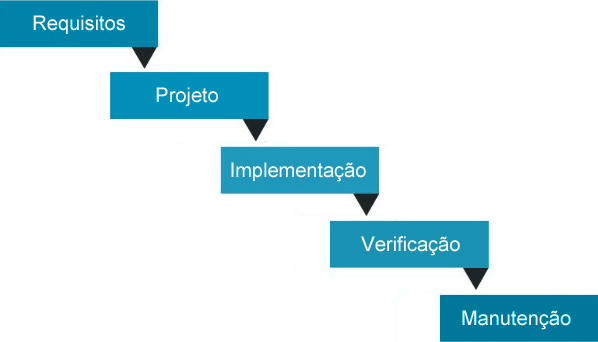
\includegraphics[width=0.6\textwidth,natwidth=598,natheight=342]{figura2.jpg}
	\end{center}
\end{figure}

A rigidez imposta por essa sequência entre as fases traz algumas desvantagens. Uma delas é que o solicitante do software só terá uma visão de como o sistema funciona somente na fase final do projeto, e caso tenha mudança em algum dos requisitos ou em alguma regra de negócio, o mesmo pode acarretar em atraso do projeto \cite{pressman2005}. Isso pode até gerar um comprometimento no orçamento inicial do projeto, já que tal mudança em uma etapa tardia pode ter um esforço elevado do pessoal que desenvolve.

Outra desvantagem é que essa natureza linear da abordagem faz com que alguns membros da equipe fiquem ociosos até que um outro membro finalize sua parte, ocasionando assim um “estado de bloqueio”. Esse estado ocorre com mais frequência na transição entre uma etapa e outra (Bradac \textit{apud} \citeonline{pressman2005}).

O modelo cascata originalmente proposto por \citeonline{royce1970} garante alguns “ciclos de realimentação”, onde o processo prevê algumas mudanças no andamento do ciclo. Em contrapartida, na maior parte da literatura da área, o modelo cascata é visto como estritamente sequencial, sendo interpretado assim como um modelo rígido.

Segundo Hanna (1995), nos dias atuais o mercado vem se tornando cada vez mais exigente e, com isso, respostas rápidas a mudanças de funcionalidades, características e informações são essenciais. Geralmente nesses tipos de aplicações o modelo cascata não é indicado.

Apesar dos problemas citados, a metodologia tradicional funciona muito bem quando os requisitos estão fortemente estabelecidos ou o produto final é uma atualização de um software já em funcionamento -- aqui somente a tecnologia irá mudar e não as funcionalidades e características do produto.

O uso da metodologia de desenvolvimento tradicional pode ser adaptada para a área de desenvolvimento de jogos. A Figura \ref{fig_gwp} mostra que as fases do processo de desenvolvimento de jogos (ver Seção \ref{sec_jogos}) segue também uma ordem sequencial, assim como visto na metodologia tradicional (ver Figura \ref{fig_cascata}) da engenharia de software. Essa adaptação é denominada na literatura como sendo \textit{Game Waterfall Process} (tradução livre, Processo Cascata de Jogo). 

\begin{figure}[!htbp]
	\begin{center}
	\caption{Game Waterfall Process}
	\label{fig_gwp}
	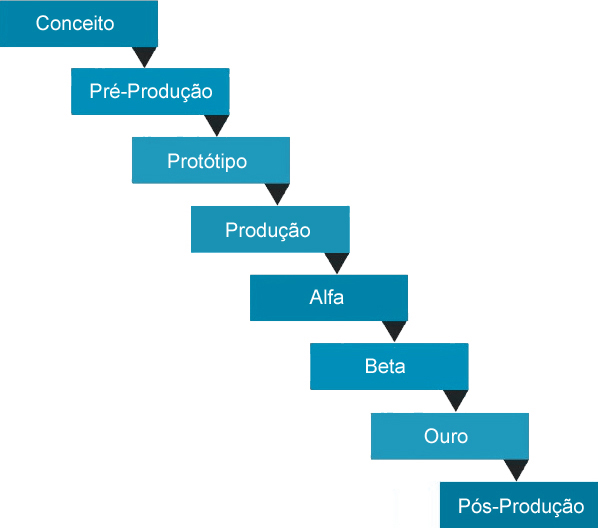
\includegraphics[width=0.6\textwidth,natwidth=598,natheight=528]{figura1.jpg}
\end{center}
\end{figure}

Nessa metodologia o princípio é o mesmo do ciclo de vida clássico, onde uma fase só começa quando a outra anterior é finalizada. Por seguir esse princípio, tal abordagem possui os mesmo problemas encontrados na abordagem cascata da engenharia de software. Segundo \citeonline{flood2003}, esse processo linear expõe as fases de diferentes pontos de vista, onde um grupo de testes só conseguirá visualizar o projeto quando o time de desenvolvimento finalizar sua etapa.


\subsection{Rational Unified Process - RUP}
\label{sec_rup}

Segundo \citeonline{kroll2003}, o Processo Unificado da Rational (RUP) é um processo de desenvolvimento de software bem estruturado e bem definido. O processo define como as tarefas são executadas, quando e por quem. Além disso, o RUP fornece uma estrutura bem definida também para o ciclo de vida de um projeto, articulando claramente os pontos de decisão.

De acordo com \citeonline{sommerville2010}, o RUP é descrito em três perspectivas, enquanto que os modelos convencionais apresentam uma visão única do processo de desenvolvimento de software. As perspectivas são:

\begin{itemize}
	\item Perspectiva dinâmica: que apresenta as fases do modelo em relação ao tempo.
	\item Perspectiva estática: apresenta as atividades a serem realizadas no processo.
	\item Perspectiva prática: propõe uma série de boas práticas para serem seguidas.
\end{itemize}

As fases da perspectiva dinâmica apresentada pelo RUP são: concepção, elaboração, construção e transição. Segundo \citeonline{almeida2006}, o processo de desenvolvimento de jogos pode ser dividido em quatro fases também, sendo essas análogas às do RUP. O autor ainda sugere que cada modelo deve ser adaptado de acordo com o projeto. A seguir tem-se as fases descritas por \citeonline{almeida2006}, comparando com as etapas de desenvolvimento de jogos apresentadas na Seção \ref{sec_jogos}:

\begin{itemize}
	\item Concepção: equivalente a etapa de conceito do desenvolvimento de jogos.
	\item Pré-produção: nesta fase tem-se a junção das etapas de pré-produção e protótipo.
	\item Produção: a etapa de produção é a mesma do processo de desenvolvimento de jogos.
	\item Pós-produção: aqui o autor incorpora as demais etapas, alfa, beta, ouro e pós-produção.
\end{itemize}

As atividades da perspectiva estática não são associadas a uma única fase, e podem ser realizadas em todo o andamento do projeto. Na Tabela \ref{tabela_rup} são descritas tais tarefas conforme apresentadas por \citeonline{sommerville2010}, e também é apresentada a única sugestão de adaptação por \citeonline{almeida2006}:

\begin{table}[h]
\centering
\caption{Tabela das atividades da perspectiva estática}
\label{tabela_rup}
\begin{tabular}{|p{30mm}|p{120mm}|}
\hline
\textbf{Atividade}                        & \textbf{Descrição} \\ \hline 
Game Design                               & A atividade original do RUP é denominada modelagem de negócios, onde os processos são modelados por meio de casos de uso. A proposta de adaptação para jogos foi substituir essa atividade pela construção de jogos, onde o jogo é planejado. \\ \hline 
Requisitos                                & Descrever quais as funcionalidades e interações do sistema, modelando e documentando os requisitos do sistema. \\ \hline 
Análise e design                          & Serve para planejar e modelar a arquitetura, componentes e sequência do projeto, ou seja, criar uma base para a implementação. \\ \hline 
Implementação                             & Consiste em gerar algo executável, em implementar os componentes do software e integrar os resultados das iterações. \\ \hline 
Teste                                     & Os testes podem ocorrer de forma iterativa conforme o andamento do projeto, isso permite encontrar e consertar erros o quanto antes. \\ \hline 
Implantação                               & Consiste em disponibilizar e instalar uma versão para o cliente utilizar. \\ \hline 
Gerenciamento de configurações e mudanças & Essa disciplina de apoio gerencia as mudanças do sistema. \\ \hline 
Gerenciamento de projetos                 & Gerenciar as mudanças do sistema como um todo é objetivo dessa disciplina de apoio. \\ \hline 
Ambiente                                  & Está relacionado com o ambiente da equipe de desenvolvimento de software, em fornecer artefatos e ferramentas adequados. \\ \hline
\end{tabular}
\end{table}

A Figura \ref{fig_rup} mostra essas duas primeiras perspectivas em um mesmo gráfico, onde é possível ver como elas se interagem ao decorrer do projeto.

\begin{figure}[!htbp]
	\begin{center}
	\caption{Perspectivas estática e dinâmica adaptado de \citeonline{almeida2006}}
	\label{fig_rup}
	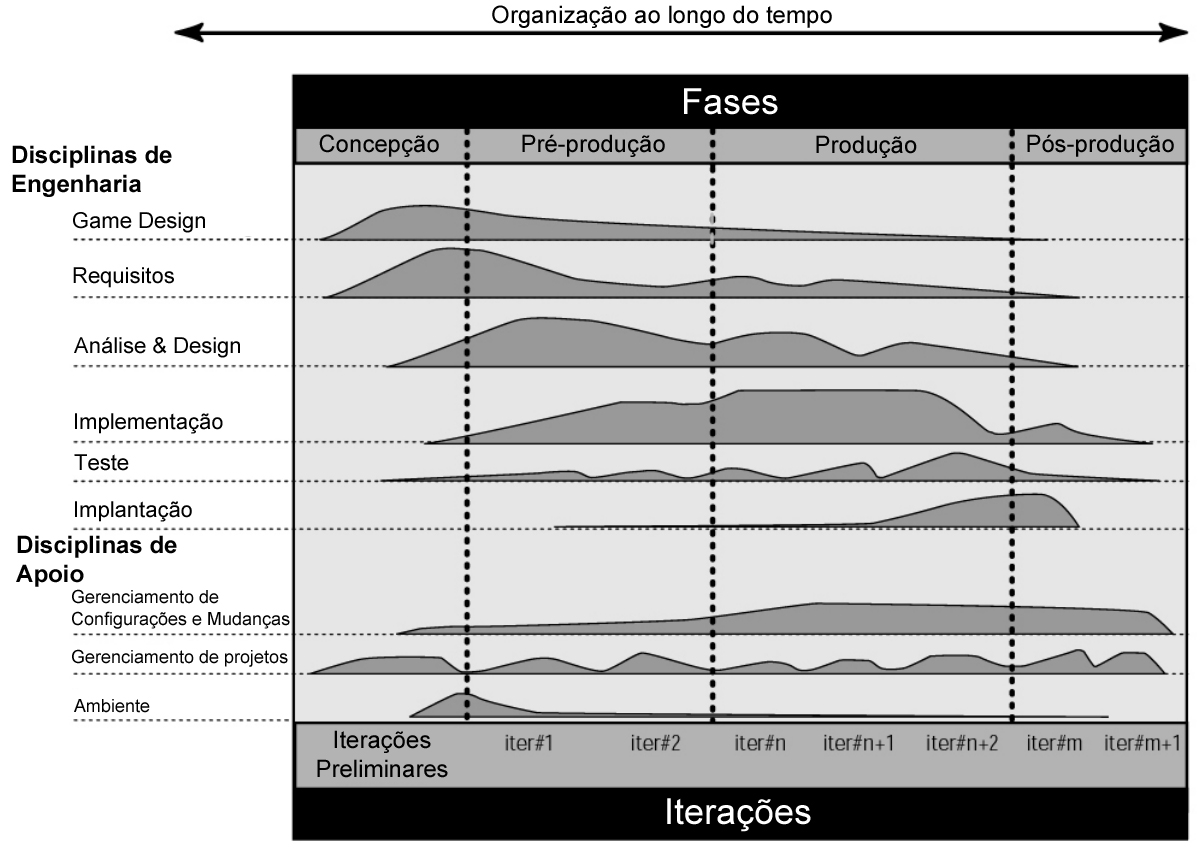
\includegraphics[width=0.8\textwidth,natwidth=1200,natheight=850]{figura5.jpg}
	\end{center}
\end{figure}

Na perspectiva prática do RUP são recomendadas algumas das práticas da engenharia de software. São seis as boas práticas fundamentais para o uso no desenvolvimento de sistemas sugeridas pelo RUP \cite{sommerville2010}:

\begin{itemize}
	\item Desenvolver software incremental e iterativamente: dividir tarefas em outras menores, planejando para que tais incrementos sejam baseados na prioridade do cliente, de forma a desenvolver primeiramente as tarefas com alta prioridade.
	\item Gerenciar requisitos: documentar todos os requisitos do sistema e suas eventuais mudanças. Permite avaliar o impacto antes de aceitar tais mudanças.
	\item Utilizar arquitetura baseada em componentes: o uso da arquitetura em componentes permite uma melhor compreensão do sistema e um melhor reaproveitamento de códigos, reduzindo assim custos e riscos.
	\item Modelar visualmente o software: para melhorar a compreensão do software para todas as partes envolvidas, modelagens visuais são mais claras e objetivas do que documentos extensos. O RUP sugere o uso da UML para modelar as etapas do desenvolvimento do projeto.
	\item Verificar a qualidade do software: garantir que a qualidade do software seja verificada continuamente por todos os envolvidos, e não somente ao final do projeto como na metodologia tradicional.
	\item Controlar as mudanças do software: utilizar sistemas e ferramentas para gerenciar as mudanças do software, de procedimentos ou configurações, já que todos os softwares estão sujeito a mudanças, principalmente no mercado de jogos.
\end{itemize}


\subsection{Metodologias ágeis}

Em meados de 2001, um grupo de dezessete especialistas se reuniu para discutir aspectos importantes sobre desenvolvimento de software. A partir daí, um conjunto de valores e princípios foram estabelecidos para nortear o processo de desenvolvimento ágil de software, criando assim o chamado manifesto ágil \cite{beck2001}.

Para a criação do manifesto, a ideia principal foi valorizar mais: indivíduos e interações do que processos e ferramentas; software em funcionamento do que documentação em excesso; colaboração com o cliente do que negociação de contratos; responder a mudanças do que seguir um plano \cite{beck2001}.

Para melhor compreensão dessa nova filosofia de desenvolvimento, o grupo também criou uma lista com doze princípios que devem ser seguidos. São eles \cite{beck2001}:

\begin{itemize}
	\item Satisfação do cliente através da entrega adiantada e contínua de software de valor.
	\item Aceitar mudanças de requisitos, mesmo no fim do desenvolvimento.
	\item Entregar software funcionando com frequência.
	\item Pessoas relacionadas a negócios e desenvolvedores devem trabalhar em conjunto e diariamente.
	\item Construir projetos com indivíduos motivados, dando ambiente e suporte necessário, e confiar que farão seu trabalho.
	\item Conversa face a face é o método mais eficiente e eficaz de transmitir informações.
	\item Software funcional é a principal medida do progresso.
	\item Desenvolvimento sustentável. Patrocinadores, usuários e desenvolvedores devem manter um ritmo constante indefinidamente.
	\item Atenção contínua à excelência técnica e bom design.
	\item Simplicidade - a arte de maximizar a quantidade de trabalho que não precisa ser feito.
	\item As melhores arquiteturas, requisitos e projetos emergem de equipes auto-organizáveis.
	\item Em intervalos regulares, a equipe deve refletir sobre como se tornar mais eficiente.
\end{itemize}

Seguindo nessa linha de pensamento, várias metodologias surgiram descritas como ágil, sendo elas: \textit{Agile Unified Process}, \textit{Test-Driven Development} (TDD), \textit{Feature-Driven Development} (FDD) e \textit{Dynamic Systems Development Method} (DSDM). Mas duas delas ganharam muitos adeptos no mercado: SCRUM e \textit{Extreme Programming} (XP) que serão detalhadas nas próximas seções.


\subsubsection{SCRUM}

SCRUM é um modelo ágil de processo que está de acordo com o manifesto ágil proposto em 2001 \cite{sommerville2010}. Em suma, essa metodologia para gerenciamento de projetos tem como característica entregar resultados de maneira incremental, efetiva e com menor custo, implementando requisitos realmente necessários. A flexibilidade e facilidade de adaptação do projeto diante das inevitáveis mudanças é um outro princípio dessa metodologia \cite{schwaber1997}. 

A inspeção e a verificação contínua do produto em desenvolvimento têm um papel importante no SCRUM. Como resultado, possíveis problemas ou correções podem ser encontrados e corrigidos o quanto antes. Outro princípio importante é manter uma equipe pequena, organizada e auto gerenciável, maximizando a comunicação e minimizando a supervisão entre os membros, ou seja, cria-se uma confiabilidade entre os membros da equipe \cite{pressman2005}.

Na metodologia SCRUM existem papéis fundamentais com o objetivo de definir a atuação de todos os participantes envolvidos em um determinado projeto. Uma esquematização de tais papéis pode ser visto na Figura \ref{fig_papeis}. Ressaltando que daqui em diante os exemplos são dados no contexto de jogos, os papéis fundamentais na metodologia SCRUM são \cite{keith2010}: 

\begin{itemize}
	\item Product Owner: é quem conhece o produto, sendo responsável por fornecer a visão do jogo solicitado e priorizar quais funcionalidades são mais importantes. Ele é o responsável por manter o Backlog do produto (\textit{Product Backlog}) sempre atualizado e priorizado.
	\item Scrum Master: possui um papel gerencial dentro do projeto, garantindo que a equipe siga adequadamente as práticas do SCRUM. Além disso, esse profissional atua como mediador de possíveis conflitos e como facilitador para eliminar os obstáculos.
	\item Scrum Team: é o time de profissionais multidisciplinares responsável por desenvolver o jogo. Geralmente é uma equipe pequena que, além de ser transfuncional (um membro pode possuir várias funções), é também auto gerenciável, onde cada membro da equipe tem o poder de organizar seu próprio trabalho.
\end{itemize}

\begin{figure}[!htbp]
	\begin{center}
	\caption{Papéis Scrum - Adaptado de \citeonline{keith2010}}
	\label{fig_papeis}
	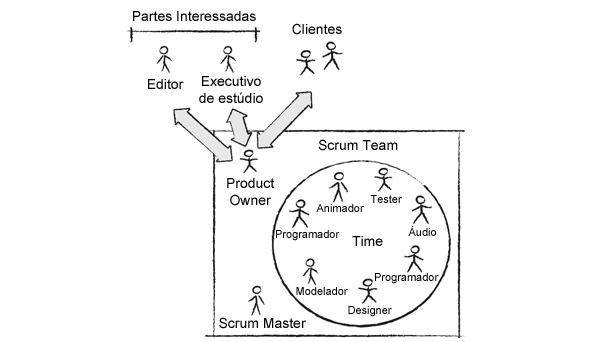
\includegraphics[width=0.8\textwidth,natwidth=598,natheight=342]{figura3.jpg}
	\end{center}
\end{figure}

A Figura \ref{fig_scrum} mostra uma abordagem geral de como funciona o SCRUM. Parte do sistema ou do jogo é apresentado de duas a quatro semanas, sendo essa entrega denominada \textit{Sprint}. No início de cada \textit{Sprint}, o time responsável pelo projeto se reúne para realizar uma reunião conhecida como \textit{Sprint Planning Meeting}. Nessa reunião eles selecionam algumas funcionalidades do \textit{Product Backlog}, que contém a lista de todas as funcionalidades do sistema já priorizada pelo cliente. Esse conjunto de funcionalidades selecionadas pelo time para ser desenvolvido é conhecido como \textit{Sprint Backlog}. Ainda nessa reunião cada item por sua vez é discutido pela equipe a fim de estimar um tempo a ser gasto no desenvolvimento de cada tarefa \cite{keith2010}. Logo abaixo tem-se uma explicação de cada um desses artefatos/eventos citados dentre outros utilizados no Scrum.

\begin{figure}[!htbp]
	\begin{center}
	\caption{Visão Geral do Scrum - Adaptado de \citeonline{keith2010}}
	\label{fig_scrum}
	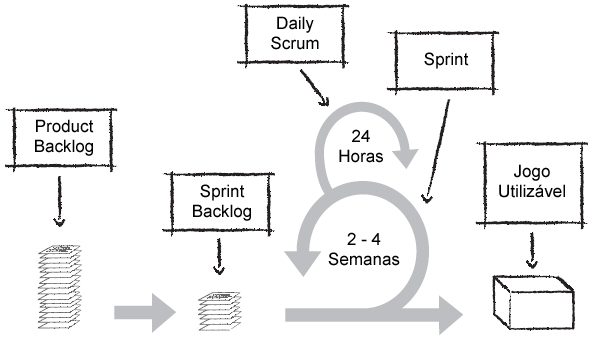
\includegraphics[width=0.8\textwidth,natwidth=598,natheight=342]{figura4.jpg}
	\end{center}
\end{figure}

Os artefatos do Scrum servem principalmente como transparência para todos os envolvidos no projeto, gerando uma flexibilidade para que todos possam inspecionar e sugerir adaptações de acordo com a dinâmica gerada no andamento do jogo.

\begin{itemize}
	\item Product Backlog: é uma lista ordenada de funcionalidades do jogo, ou seja, tudo o que fará parte do jogo deve estar nessa lista. O responsável por manter essa lista priorizada e completa é do \textit{Product Owner}. Uma característica do \textit{Product Backlog} é ser uma lista dinâmica, pois alterações podem aparecer constantemente para deixar o jogo sempre útil, atrativo e competitivo.
	\item Sprint Backlog: é um conjunto de funcionalidades do \textit{Product backlog}, tais funcionalidades deverão serão entregues ao final da \textit{Sprint}. O time de desenvolvimento é responsável por manter essa lista sempre atualizada, mostrando quais tarefas já foram executadas, quais estão com algum impedimento e quais ainda estão na fila. Essa lista também é dinâmica, já que algumas tarefas podem demandar outras tarefas não previstas.
	\item Incremento: é o resultado da \textit{Sprint} como uma versão potencialmente utilizável, é a soma dos itens do \textit{Product Backlog} que já foram executados, ou seja, o resultado da \textit{Sprint} atual somado com as \textit{Sprints} anteriores.
\end{itemize}

De acordo com \citeonline{schwaber2016}, dentro da metodologia Scrum existem alguns eventos definidos para nortear a execução do projeto, permitindo uma melhor transparência e inspeção por parte de todos os participantes. Os eventos do Scrum são:

\begin{itemize}
	\item Sprint: em um projeto de desenvolvimento utilizando Scrum, uma versão potencialmente utilizável é entregue no final de cada \textit{Sprint}, dando início a \textit{Sprint} seguinte. Por isso é conhecida como o coração do Scrum. É onde acontecem os demais eventos e geralmente tem duração fixa de um mês ou menos. 
	\item Sprint Planning: é uma reunião que acontece sempre ao início de cada \textit{Sprint}, geralmente é dividida em duas etapas. Na primeira, o \textit{Product Owner} define quais itens do \textit{Product Backlog} deverá ser implementado, definindo o objetivo principal da \textit{Sprint}. Tendo a lista dos itens que serão entregues na \textit{Sprint} (\textit{Sprint Backlog}), o time começa a definir como irá construir tais funcionalidades, dividindo cada item em tarefas e dando um prazo para cada uma, transformando-os em incremento do produto no final da \textit{Sprint}.
	\item Daily Scrum: todos os dias o time Scrum se reúne para trocar informações sobre o andamento da \textit{Sprint} e sobre o que se pretende fazer até a próxima reunião. Essa é uma reunião rápida, geralmente de 15 minutos, onde todos respondem a três perguntas: o que fiz da última reunião até agora que ajudou na meta da \textit{Sprint}? O que farei hoje para atender a meta? Existe algum impedimento que precisa ser resolvido para atender a meta? Esses pontos servem para melhorar o sincronismo e a comunicação do time de desenvolvimento.
	\item Sprint Review: é uma revisão realizada ao final de cada \textit{Sprint}. Geralmente as partes interessadas se reúnem junto com o time de desenvolvimento para inspecionar e colaborar com o incremento realizado. Se necessário, o \textit{Product Owner} aproveita essa reunião para ajustar o \textit{Product Backlog}.
	\item Retrospective: após a revisão da \textit{Sprint}, o time de desenvolvimento realizada uma reunião de retrospectiva, levantando os principais pontos positivos e negativos do time. Esses pontos estão ligados ao relacionamento com os integrantes do time, às ferramentas e aos processos, e servem para criar um plano de melhorias a serem aplicadas na \textit{Sprint} seguinte.
\end{itemize}


\subsubsection{Extreme Game Development - XGD}

O \textit{Extreme Game Development} (XGD) é definido como uma metodologia ágil para o desenvolvimento de jogos. Como o próprio nome sugere, essa metodologia foi elaborada utilizando como base os princípios e valores da metodologia \textit{Extreme Programming} (XP) \cite{demachy2003}.

Muitas equipes de desenvolvimento de jogos utilizam o XP como metodologia padrão. Mas como o XP foi criado para facilitar a vida dos programadores, com artefatos e processos voltados para desenvolvedores, tal metodologia precisou de uma pequena adaptação para facilitar o entendimento no ambiente de desenvolvimento de jogos, uma vez que existem pessoas de diversas disciplinas trabalhando em um mesmo projeto \cite{demachy2003}.

O modelo XGD baseia-se nos cinco princípios ou valores básicos da metodologia XP, que são definidos por \citeonline{beck2000}: 

\begin{itemize}
	\item Comunicação: todos são parte do time, e a comunicação diária é de extrema importância para o sucesso do projeto. A comunicação deve ser entre os membros do time de desenvolvimento e também da equipe com o cliente. Assim, todos os pontos importantes podem ser tratados com a agilidade e atenção que merecem.
	\item Feedback: a atuação do cliente é essencial para que possíveis alterações ou melhorias possam ser efetuadas o quanto antes. Quanto mais o cliente aprende com o produto, maior deve ser seu feedback ao time de desenvolvimento, pois assim a equipe pode focar em algo que realmente agregue valor ao cliente.
	\item Simplicidade: o foco é entregar somente o funcional e o mais simples possível. Isso agregará valor ao cliente, uma vez que ele vê o investimento dele em algo palpável.
	\item Coragem: dizer sempre a verdade sobre estimativas e andamento do projeto, encarar as mudanças assim que elas surgirem, e apoiar toda equipe, pois ninguém trabalha sozinho.
	\item Respeito: todos são responsáveis pelo projeto, então cabe a cada um respeitar a diversidade, o nível de conhecimento e as limitações do outro.
\end{itemize}

Um ponto importante do XGD é que manteve a maioria das práticas aplicadas no XP. Tais práticas auxiliam todos os envolvidos no projeto a manterem sempre em mente os valores mencionados acima. Algumas dessas práticas são \cite{teles2014}:

\begin{itemize}
	\item Cliente presente: A participação ativa do cliente é essencial para obter o máximo de valor do projeto. Com essa participação ativa, o feedback entre as partes torna-se mais efetivo, viabilizando maior simplicidade no processo de desenvolvimento.
	\item Jogo do planejamento: No início de cada release (módulos do sistema que serão entregues por etapas) e cada iteração (período de tempo que a equipe desenvolve um conjunto de funcionalidades) ocorre o jogo do planejamento, onde o cliente avalia as funcionalidades que serão implementas, e a equipe faz uma estimativa do custo da implementação.
	\item Stand up meeting: Traduzindo tem-se reunião em pé. É uma reunião rápida que acontece todos os dias pela manhã com o time de desenvolvimento. Nela, a equipe avalia o trabalho executado no dia anterior, e prioriza o que será implementado no decorrer do dia.
	\item Programação em par: A ideia é colocar dois programadores em um mesmo computador para produzir o mesmo código. Nesta prática, o código produzido já é revisado em sua construção. Isso permite também que o código seja mais simples e eficaz, pois há uma troca de experiências a todo momento entre os desenvolvedores.
	\item Refactoring: Refatorar é o ato de refazer um código sem alterar sua funcionalidade. É utilizado para que o código gerado fique sempre claro e objetivo, facilitando assim a manutenção do mesmo.
	\item Código coletivo: Diferentemente de outras metodologias, onde cada desenvolvedor é responsável por uma parte do sistema, no XP todos tem acesso a todas as partes do sistema, e podem alterar aquilo que julgarem importante. Cria-se assim mais uma opção de revisão de código, além de fornecer uma maior agilidade no processo.
	\item Design simples: A equipe é focada em desenvolver códigos simples para atender às necessidades da funcionalidade que está implementando, sem criar algorítimos complexos. Eles contam com a prática de refatoração quando precisarem incorporar qualquer necessidade futura.
	\item Integração contínua: Para que o sistema esteja sempre funcionando ao se incorporar uma nova funcionalidade, a equipe realiza a prática de integração contínua, adequando os códigos gerados com o restante do sistema.
	\item Releases curtos: Um conjunto de funcionalidades é colocado em produção em um curto espaço de tempo, para que o cliente já possa utilizar e gerar seu feedback. Com isso, o sistema é colocado em produção diversas vezes ao longo do projeto, gerando mais valor e incorporando mais funcionalidades a cada release.
\end{itemize}

Com essas e outras práticas existentes na metodologia XP, o XGD torna-se uma opção promissora no que diz respeito a desenvolvimento de jogos. Porém, devido a sua filosofia de manter o mais simples possível, a falta de documentação necessária pode vir a ser um problema. Pensando nisso, \citeonline{flood2003} propôs uma metodologia híbrida que será descrita a seguir.


\subsubsection{Game Unified Process - GUP}

\citeonline{flood2003}, um gerente de projetos da área de jogos criou o processo denominado \textit{Game Unified Process} (GUP) em 2003, baseado em sua experiência gerencial no desenvolvimento de jogos. Em vários projetos observou-se alguns problemas constantes, que poderiam ser evitados, pois tais problemas são comuns conhecidos da metodologia cascata utilizada até então, e já citados na Seção \ref{sec_cascata}. 

Para sanar tais problemas ele decidiu criar essa metodologia híbrida, combinando características do RUP e XP. O propósito foi utilizar a documentação detalhado e os ciclos longos do RUP juntamente com algumas práticas do XP como trabalhar com times pequenos, focado em entregas pequenas e seus ciclos curtos.

Além dos problemas com a metodologia tradicional, um dos argumentos que os desenvolvedores citavam era que os artistas se sentiam constrangidos pelo processo engessado que era utilizado.  Eles sentiam que não podiam mostrar seu verdadeiro potencial de criatividade quando surgia uma oportunidades, devido ao ambiente extremamente estruturado \cite{flood2003}.

\citeonline{flood2003} não faz um detalhamento de como a metodologia funciona. Entende-se que o autor quis deixar seu ponto de vista de que o desenvolvimento de jogos não é um procedimento linear, e que processos ágeis e incrementais podem ser alternativas efetivas para o mundo dos jogos. Além disso, ele mostra que as vezes uma única metodologia pode não ser suficiente, e que a combinação de pontos positivos de algumas metodologias pode ser uma saída.


\section{Métricas}

Para discutir as possíveis métricas que possam ser utilizadas nesse trabalho, é preciso definir o conceito da mesma. Segundo \citeonline{ieee1990}, métrica é um método para determinar se um sistema, componente ou processo possui um determinado atributo. \citeonline{sommerville2010} define uma métrica de software como sendo uma característica de um sistema, processo de desenvolvimento ou documentação que pode ser medida objetivamente. Tais métricas são essenciais na construção de um software, pois elas são responsáveis por aferir a qualidade do projeto.

De acordo com \citeonline{sommerville2010}, as metricas de software podem ser divididas em duas visões: métricas de controle e métricas de previsão. A primeira pode ser utilizada para avaliar o processo de desenvolvimento de um projeto, enquanto a segunda pode ser utilizada para avaliar atributos internos do produto.

As métricas de previsão geralmente são utilizadas para analisar dados referente ao produto, e são dados que uma pessoa externa à empresa normalmente não tem acesso, como quantidade de linhas de códigos, total de defeitos encontrados, custo, número de casos de uso, número de classes, entre outros \cite{guarizzo2008}. 

Com as métricas de controle é possível analisar a qualidade do processo de desenvolvimento \cite{pressman2005}, como a facilidade ou não de um processo conseguir realizar a menutenção de uma certa funcionalidade, tempo dedicado em uma etapa específica da produção de jogos, entre outros.

Uma vez que o intuito deste trabalho é analisar as metodologias de desenvolvimento voltado para jogos, as métricas de previsão não serão tão exploradas durante o andamento do projeto. Porém algumas métricas de controle serão utilizadas, para tentar levantar alguns dados como número de erros após o jogo implantado, quantidade de funcionalidades alteradas após a conclusão da fase de conceito e pré-produção, entre outros. Tudo isso para garantir um melhor aproveitamento no processo de desenvolvimento.

% Número de erros após o jogo implantado
% Quantidade de funcionalidades alteradas/incluídas após concluído a fase de conceito e pré-produção
% Quantidade de estórias que foram implementadas no sprint (para ágeis)
% Funcionalidade testada e entregue, tempo médio do ciclo


\section{Trabalhos Relacionados}

Nesta seção será apresentado alguns trabalhos que compararam algumas das metodologias de desenvolvimento voltado para jogos.

Um dos trabalhos é apresentado por \citeonline{araujo2006}, cujo o intuito é sugerir uma nova abordagem de desenvolvimento com base nas melhotas práticas de outras metodologias, para melhor adequar a produção de jogos publicitários. 

As metodologias que o autor apresenta em seu estudo são: \textit{Waterfall}, Processo Unificado, \textit{Extreme Programming} e Scum. Para obter o resultado necessário ele utiliza alguns critérios para avaliar tais metodologias. Esses critérios foram: flexibilidade, comunicação, suporte a multidisciplinaridade, gerenciamento descentralizado, tratamento de riscos, valor e suporte ao desenvolvimento. Com isso ele classifica cada critério para cada metodologia em quatro níveis (fraco, regular, bom e ótimo).

Após a análise das metodologias existentes, \citeonline{araujo2006} conclui que nenhuma metodologia é completamente aderente às necessidades de um projeto \textit{advergame} (integração de propaganda e jogos eletrônicos), e propõe uma nova abordagem, denominada \textit{Agile Game Process} (AGP). A essência dessa metodologia é utilizar os valores descritos pelo Manifesto Ágil \cite{beck2001}, com isso ele uniu os mecanismos gerenciais do Scrum com as práticas de desenvolvimento do XP. Além disso, o autor define o processo de desenvolvimento em três fases (Concepção, Construção e Pós-Construção), e define algumas disciplinas que cada ciclio deve seguir, tornando similar ao gráfico do RUP apresentado na Seção \ref{sec_rup}.

Outro trabalho relacionado é o de \citeonline{barros2007}, que fez uma análise de algumas metodologias de desenvolvimento voltada para jogos. Ele analisou as principais metodologias encontradas na literatura e também as utilizadas por empresas da região de Pernambuco. Como resultado da análise, o autor propõe um “Manual de Boas Práticas para Desenvolvimento de Jogos”, cujo o intuito é auxiliar empresas iniciantes no desenvolvimento de jogos.

Dentre as metodologias que o autor analisa na literatura encontram-se: \textit{Game Waterfall Process}, \textit{Extreme Game Development}, \textit{Game Unified Process} e SCRUM. Para obter o resultado necessário ele utiliza os mesmos critérios definidos por \citeonline{araujo2006} para avaliar as metodologias de desenvolvimento de jogos.

Após essa avaliação, o autor realiza uma pesquisa com três empresas locais de Pernambuco, a fim de obter informações sobre definições e práticas utilizadas. Um questionário é enviado para alguns gerentes e desenvolvedores dessas empresas para a coleta de tais informações. Apesar de resultados interessantes, uma gama pequena de empresas foram consultadas. 

Como resultado do trabalho, \citeonline{barros2007} apresenta uma lista com cinco artefatos, nove práticas e sete papéis sugeridos para o desenvolvimento de jogos.

% Talvez citar as diferenças existentes entre os trabalhos relacionados e o meu projeto!!?
%
% Neste trabalho é apresentado um estudo das metodologias citadas pelos autores acima, com uma ênfase maior no desenvolvimento de jogos.


\section{Considerações finais}

O uso de metodologias de desenvolvimento é algo essencial para o sucesso de qualquer projeto, desde o mais simples ao mais complexo. Porém a escolha da melhor metodologia depende de cada empresa, de cada projeto e de cada equipe. O objetivo deste capítulo foi apresentar o maior número de metodologias que podem ser utilizadas para o desenvolvimento de jogos. Neste contexto, foram apresentadas, inicialmente, informações sobre a realidade do mercado de TI. Em seguida, foram apresentadas os principais conceitos envolvendo o desenvolvimento de jogos eletrônicos (Seção \ref{sec_jogos}). Depois foram discutidas as principais abordagens para desenvolvimento de tais jogos (Seção \ref{sec_metodologias}) e, logo após, uma breve descrição sobre métricas foi apresentado. Por fim tem-se uma breve abordagem de alguns trabalhos relacionados.

No próximo capítulo será descrito qual o propósito deste trabalho, quais métricas serão utilizadas para avaliar as metodologias aqui descritas, como coletar os dados junto às mais diversas empresas de desenvolvimento de jogos, e qual o resultado esperado dessa análise.




\chapter{Proposta do trabalho}
\label{cap_3}

\section{Considerações iniciais}

Este capítulo aborda as próximas etapas do trabalho, as quais são constituídas pelo: i) levantamento mais aprofundado das metodologidas de desenvolvimento voltadas para jogos, a fim de extrair algumas métricas para elaboração de um questionário; ii) a metodologia detalhada para fazer o levantamento dos dados e os resultados esperados.


\section{Proposta}

A proposta deste trabalho de mestrado é melhorar a qualidade do processo de desenvolvimento de jogos realizando um estudo comparativo entre as diferentes metodologias encontradas. Para o estudo comparativo, serão analisadas as metodologias de desenvolvimento de jogos eletrônicos encontrados na literatura acadêmica, as quais serão contrapostas com as metodologias empregadas na prática utilizadas em empresas e em grupos de pesquisa que desenvolvem jogos. Para obter tais informações de uso das metodologias na prática, será elaborado um questionário, que por sua vez terá como base algumas métricas encontradas na literatura. Por fim, tal comparação será utilizada para verificar similaridades, respectivas vantagens e desvantagens, tendências e padrões para cada uma das visões. 

Essa proposta tem como objetivos:

\begin{itemize}
	\item Verificar quais etapas das metodologias de desenvolvimento de jogos são comumente utilizadas nas empresas e meio acadêmico e qual o motivo do uso das mesmas. Caso tenha alguma etapa inviável de alguma metodologia, verificar o motivo dessa inviabilidade.
	\item Utilizar métricas já conhecidas na literatura para avaliar as metodologias, e caso necessário, propor melhorias de tais métricas conforme o andamento do projeto.
	\item Comparar detalhadamente as metodologias encontradas na literatura, utilizando as mé\-tri\-cas citadas acima, e contrapor com as metodologias empregadas na prática tanto na área acadêmica quando no setor privado.
	\item Propor adaptações das etapas ou artefatos das metodologias (ágeis ou não) discutidas neste trabalho.
	\item Verificar e documentar as tendências de desenvolvimento de jogos, tanto na literatura, quanto na prática (setor privado e acadêmico), a fim de melhorar o processo de desenvolvimento de jogos.
\end{itemize}


\section{Metodologia de desenvolvimento do trabalho}
\label{sec_proposta}

Nesta seção será apresentada a metodologia referente à proposta do projeto, assim como as etapas detalhadas necessárias para a realização da mesma. Tais etapas estão descritas a seguir e representadas na Figura \ref{fig_proposta}. 

\begin{figure}[!htbp]
	\begin{center}
	\caption{Etapas da proposta do projeto}
	\label{fig_proposta}
	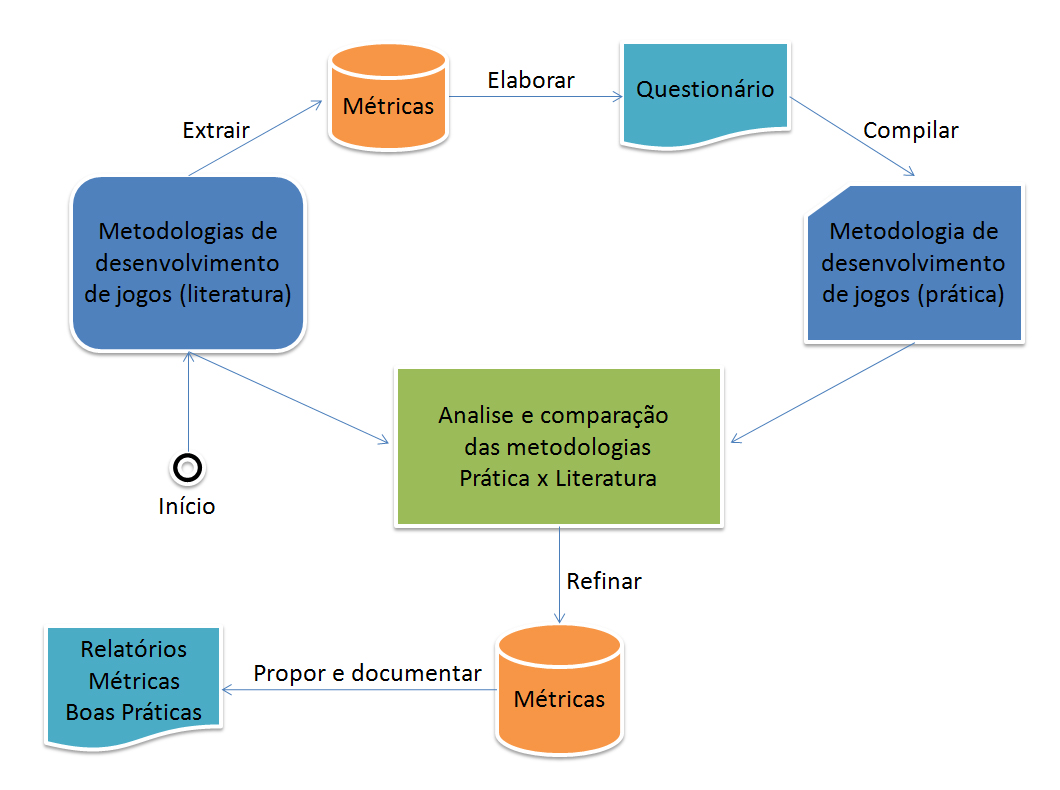
\includegraphics[width=0.8\textwidth,natwidth=1060,natheight=790]{figura6.jpg}
	\end{center}
\end{figure}

Inicialmente, será efetuado um estudo detalhado de todas as técnicas e metodologias de desenvolvimento de jogos eletrônicos encontradas na literatura (etapa inicial da Figura \ref{fig_proposta}). Para sumarizar este estudo, serão compiladas as informações obtidas por meio de tabelas e/ou gráficos, para cada uma das metodologias empregadas. Na segunda etapa ocorrerá o levantamento das métricas comumente encontradas para todas as metodologias. 

Com base nas métricas encontradas, será elaborado um questionário a ser aplicado em empresas que tenha como finalidade o ramo de desenvolvimento de jogos eletrônicos. Tal questionário será disponibilizado por meio eletrônico (website), no qual um representante da equipe de desenvolvimento será responsável por respondê-lo. 

Após a aplicação do questionário, essas informações serão compiladas e utilizadas a posteriori para realizar análise e comparação das metodologias de desenvolvimento de jogos. Após essa etapa de análise, um refinamento das métricas poderá ser realizado dependendo do resultado apresentado.

Por fim, como resultado, será proposto em um primeiro momento possíveis adaptações das metodologias de desenvolvimento (com base nos resultados anteriores), assim como gerar uma documentação das tendências de metodologias e artefatos voltadas para o desenvolvimento de jogos, tanto na literatura acadêmica quanto no mercado de trabalho.

Um exemplo de como o questionário está sendo elaborado encontra-se no Anexo \ref{anexo1}.

%
%Algumas empresas: iMax, Muve Digital, Aptor Software, Criar Games, ...
%
%Alguns grupos de desenvolvimento de jogos da academia: LOA (UFSCar), FOG (USP), USPGameDev (USP), ...
%
% Para o questionário
% - geralmente há atraso do cronograma inicialmente definido?
% - 


\section{Cronograma}

O trabalho está representado nas seguintes etapas:

\begin{enumerate}
	\item Estudo das metodologias e extração das métricas.
	\item Elaboração e aplicação do questionário.
	\item Compilação e comparação dos resultados obtidos.
	\item Proposta e documentação de melhorias e tendências.
	\item Escrita e submissão de artigos.
	\item Escrita da dissertação.
	\item Defesa da dissertação.
\end{enumerate}

\begin{table}[!ht]
\centering
\caption{Cronograma de atividades do projeto de mestrado}
\label{tabela_cronograma}
\begin{tabular}{|c|c|c|c|c|c|c|c|c|c|c|c|c|}
\hline
\multirow{2}{*}{Atividades} & 2016 & \multicolumn{11}{c|}{2017}                  \\ \cline{2-13} 
                            & 12   & 1 & 2 & 3 & 4 & 5 & 6 & 7 & 8 & 9 & 10 & 11 \\ \hline
1                           & X    & X & X &   &   &   &   &   &   &   &    &    \\ \hline
2                           &      &   & X & X &   &   &   &   &   &   &    &    \\ \hline
3                           &      &   &   &   & X & X & X &   &   &   &    &    \\ \hline
4                           &      &   &   &   &   &   & X & X &   &   &    &    \\ \hline
5                           &      &   &   &   &   &   &   & X & X &   &    &    \\ \hline
6                           &      &   &   &   &   &   &   &   & X & X & X  &    \\ \hline
7                           &      &   &   &   &   &   &   &   &   &   &    & X  \\ \hline
\end{tabular}
\end{table}

%% coloque aqui o seu arquivo .bib
%% IMPORTANTE: nao use bibliographystyle!
%% o estilo ja vem definido.
\bibliography{references}


\anexo

\chapter{Exemplo de possível questionário online}
\label{anexo1}

Neste anexo encontram-se 3 figuras para exemplificar como será elborado o questionário. Pela simplicidade e facilidade de uso, a princípio a ferramenta utilizada será o formulário do Google \footnote{Google Forms: https://www.google.com/forms/about/}. As questões serão melhor estudadas e elaboradas conforme descrito na Seção \ref{sec_proposta}.

\begin{figure}[!htbp]
	\begin{center}
	\caption{Primeira página do questionário}
	\label{fig_anexoa1}
	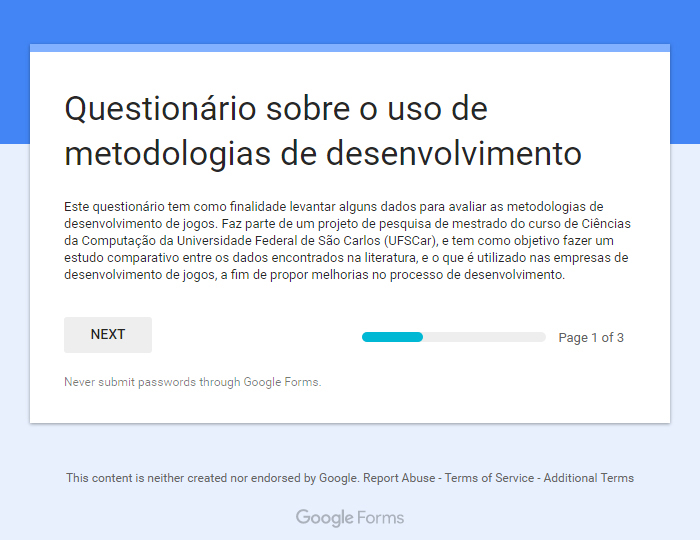
\includegraphics[width=0.9\textwidth,natwidth=700,natheight=540]{anexoA1.jpg}
	\end{center}
\end{figure}

\begin{figure}[!htbp]
	\begin{center}
	\caption{Segunda página do questionário}
	\label{fig_anexoa2}
	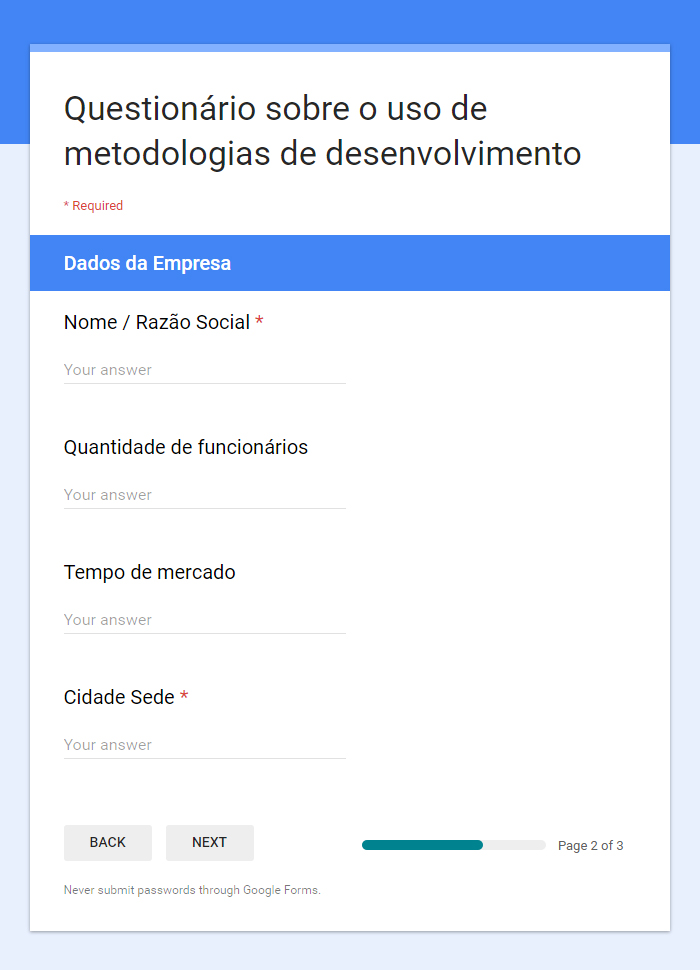
\includegraphics[width=0.9\textwidth,natwidth=700,natheight=970]{anexoA2.jpg}
	\end{center}
\end{figure}

\begin{figure}[htbp]
	\begin{center}
	\caption{Terceira página do questionário}
	\label{fig_anexoa3}
	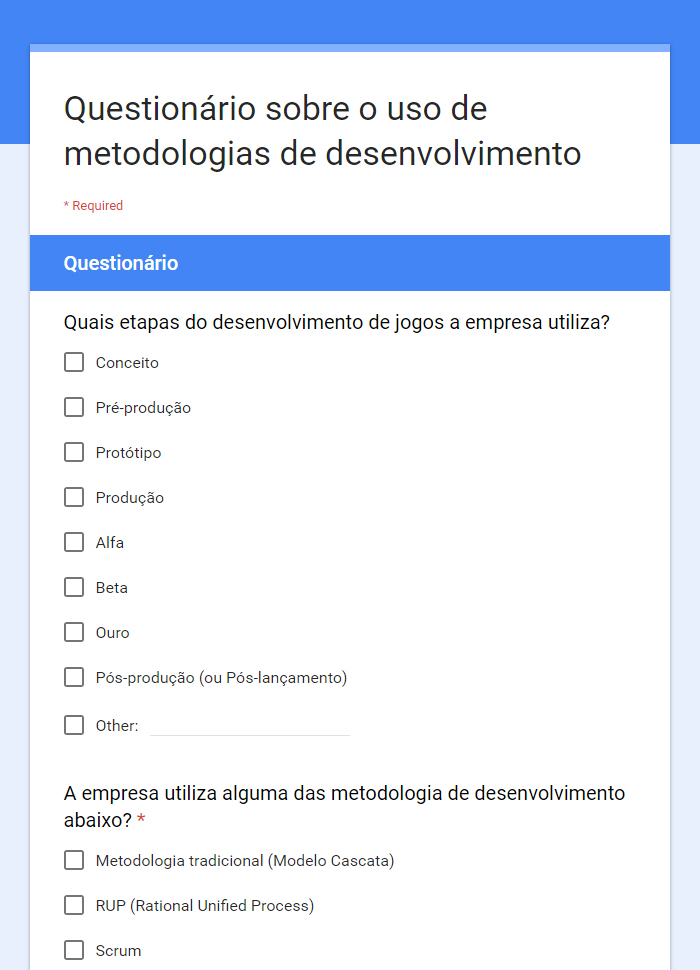
\includegraphics[width=0.9\textwidth,natwidth=700,natheight=970]{anexoA3.jpg}
	\end{center}
\end{figure}

\end{document}